\begin{comment}
\end{comment}

\begin{center}
\thispagestyle{empty}
%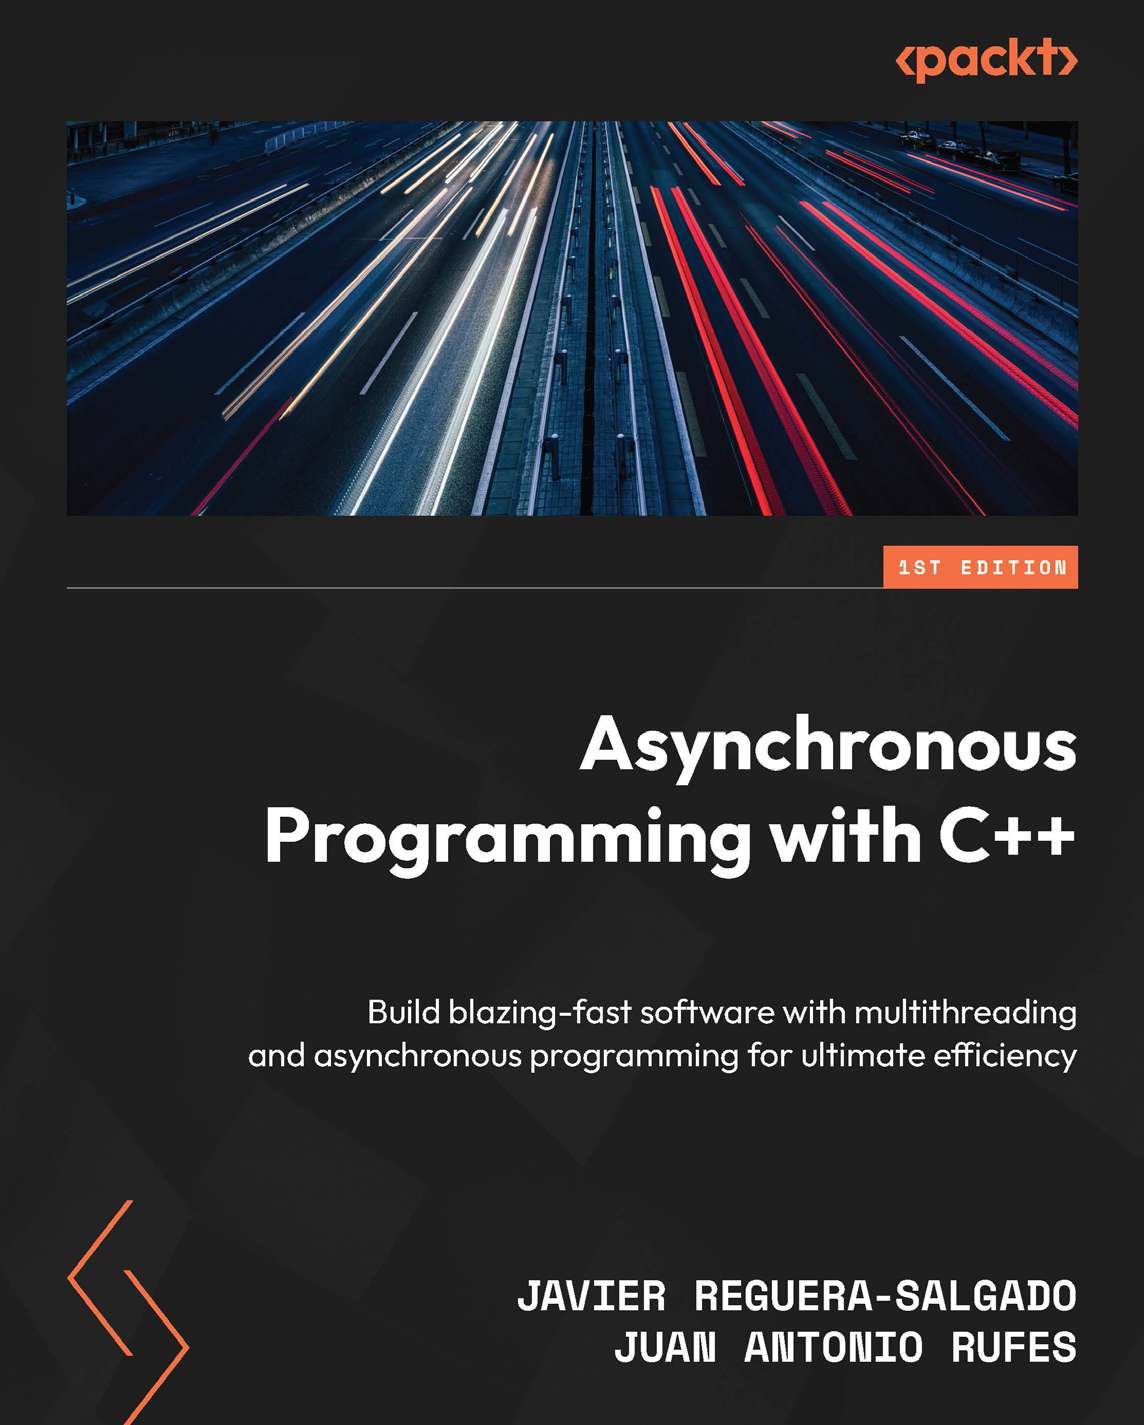
\includegraphics[width=\textwidth,height=\textheight,keepaspectratio]{cover.png}
\begin{tikzpicture}[remember picture, overlay, inner sep=0pt]
\node at (current page.center)
{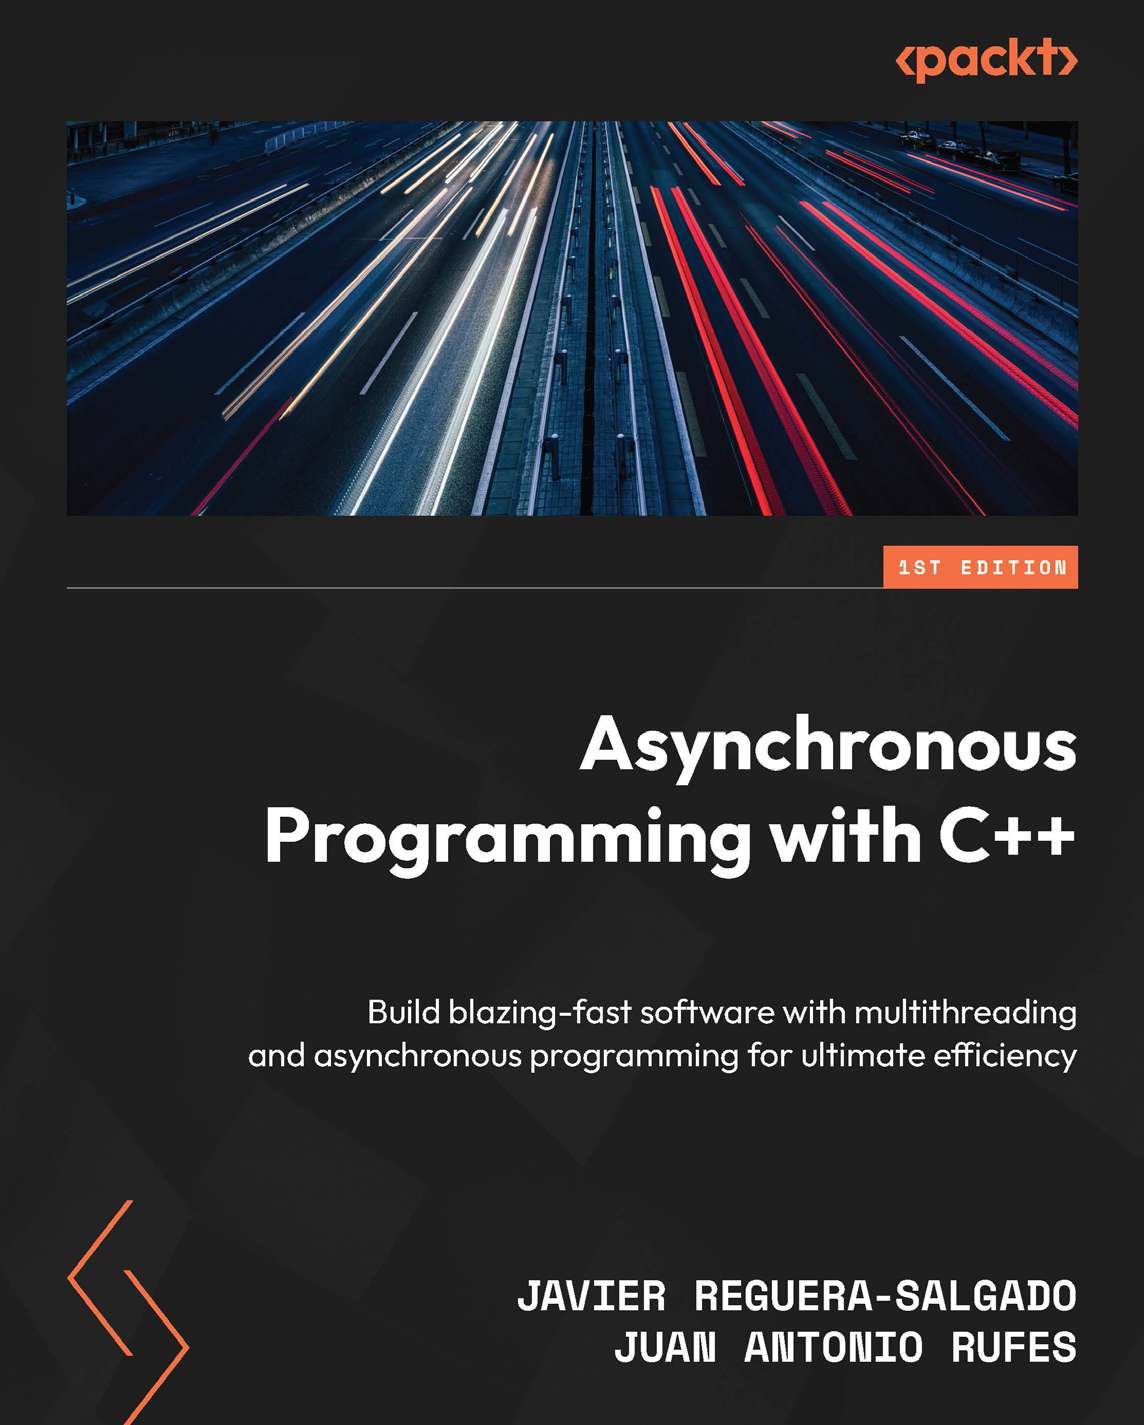
\includegraphics[width=\paperwidth, keepaspectratio=false]{cover.png}};
\end{tikzpicture}
\newpage
\thispagestyle{empty}
\huge
\textbf{Asynchronous Programming with C++}
\\[9pt]
{\Large 通过多线程和异步编程打造高速运行的软件}
\\[9pt]
\normalsize
作者: Javier Reguera-Salgado / Juan Antonio Rufes
\\[8pt]
\normalsize
译者:\href{https://github.com/xiaoweiChen/Asynchronous-Programming-with-Cpp}{陈晓伟}
\\[8pt]
\end{center}

\newpage

\pagestyle{empty}
\tableofcontents
\newpage

\setsecnumdepth{section}

\myChapter{}{前言}{content/Preface.tex}
\newpage

\myPartGray{第一部分}{Foundations of Parallel Programming and Process Management}{content/part1/part.tex}
\newpage

\myChapter{第1章}{Parallel Programming Paradigms}{content/part1/chapter1/0.tex}
\mySubsection{1.1.}{Technical requirements}{content/part1/chapter1/1.tex}
\mySubsection{1.2.}{Getting to know classifications, techniques, and models}{content/part1/chapter1/2.tex}
\mySubsection{1.3.}{Understanding various parallel programming paradigms}{content/part1/chapter1/3.tex}
\mySubsection{1.4.}{Exploring the metrics to assess parallelism}{content/part1/chapter1/4.tex}
\mySubsection{1.5.}{总结}{content/part1/chapter1/5.tex}
\mySubsection{1.6.}{扩展阅读}{content/part1/chapter1/6.tex}
\newpage

\myChapter{第2章}{Parallel Programming Paradigms}{content/part1/chapter2/0.tex}
\mySubsection{1.1.}{Processes in Linux}{content/part1/chapter2/1.tex}
\mySubsection{1.2.}{Services and daemons in Linux}{content/part1/chapter2/2.tex}
\mySubsection{1.3.}{Threads}{content/part1/chapter2/3.tex}
\mySubsection{1.4.}{Synchronization primitives}{content/part1/chapter2/4.tex}
\mySubsection{1.5.}{Common problems when using multiple threads}{content/part1/chapter2/5.tex}
\mySubsection{1.6.}{Strategies for effective thread management}{content/part1/chapter2/6.tex}
\mySubsection{1.7.}{总结}{content/part1/chapter2/7.tex}
\mySubsection{1.8.}{扩展阅读}{content/part1/chapter2/8.tex}
\newpage

\myPartGray{第二部分}{Foundations of Parallel Programming and Process Management}{content/part2/part.tex}
\newpage

\myChapter{第3章}{How to Create and Manage Threads in C++}{content/part2/chapter3/0.tex}
\mySubsection{3.1.}{Technical requirements}{content/part2/chapter3/1.tex}
\mySubsection{3.2.}{The thread library – an introduction}{content/part2/chapter3/2.tex}
\mySubsection{3.3.}{Thread operations}{content/part2/chapter3/3.tex}
\mySubsection{3.4.}{Thread-local storage}{content/part2/chapter3/4.tex}
\mySubsection{3.5.}{Implementing a timer}{content/part2/chapter3/5.tex}
\mySubsection{3.6.}{总结}{content/part2/chapter3/6.tex}
\mySubsection{3.7.}{扩展阅读}{content/part2/chapter3/7.tex}
\newpage

\myChapter{第4章}{Thread Synchronization with Locks}{content/part2/chapter4/0.tex}
\mySubsection{4.1.}{Technical requirements}{content/part2/chapter4/1.tex}
\mySubsection{4.2.}{Understanding race conditions}{content/part2/chapter4/2.tex}
\mySubsection{4.3.}{Why do we need mutual exclusion?}{content/part2/chapter4/3.tex}
\mySubsection{4.4.}{Generic lock management}{content/part2/chapter4/4.tex}
\mySubsection{4.5.}{Condition variables}{content/part2/chapter4/5.tex}
\mySubsection{4.6.}{Implementing a multithreaded safe queue}{content/part2/chapter4/6.tex}
\mySubsection{4.7.}{Semaphores}{content/part2/chapter4/7.tex}
\mySubsection{4.8.}{Barriers and latches}{content/part2/chapter4/8.tex}
\mySubsection{4.9.}{Performing a task only once}{content/part2/chapter4/9.tex}
\mySubsection{4.10.}{总结}{content/part2/chapter4/10.tex}
\mySubsection{4.11.}{扩展阅读}{content/part2/chapter4/11.tex}
\newpage

\myChapter{第5章}{Atomic Operations}{content/part2/chapter5/0.tex}
\mySubsection{5.1.}{Technical requirements}{content/part2/chapter5/1.tex}
\mySubsection{5.2.}{Introduction to atomic operations}{content/part2/chapter5/2.tex}
\mySubsection{5.3.}{Non-blocking data structures}{content/part2/chapter5/3.tex}
\mySubsection{5.4.}{The C++ memory model}{content/part2/chapter5/4.tex}
\mySubsection{5.5.}{C++ Standard Library atomic types and operations}{content/part2/chapter5/5.tex}
\mySubsection{5.6.}{SPSC lock-free queue}{content/part2/chapter5/6.tex}
\mySubsection{5.7.}{总结}{content/part2/chapter5/7.tex}
\mySubsection{5.8.}{扩展阅读}{content/part2/chapter5/8.tex}
\newpage

\myPartGray{第三部分}{Foundations of Parallel Programming and Process Management}{content/part3/part.tex}
\newpage

\myChapter{第6章}{Promises and Futures}{content/part3/chapter6/0.tex}
\mySubsection{6.1.}{Technical requirements}{content/part3/chapter6/1.tex}
\mySubsection{6.2.}{Exploring promises and futures}{content/part3/chapter6/2.tex}
\mySubsection{6.3.}{The benefits and drawbacks of promises and futures}{content/part3/chapter6/3.tex}
\mySubsection{6.4.}{Examples of real-life scenarios and solutions}{content/part3/chapter6/4.tex}
\mySubsection{6.5.}{总结}{content/part3/chapter6/5.tex}
\mySubsection{6.6.}{扩展阅读}{content/part3/chapter6/6.tex}
\newpage

\myChapter{第7章}{The Async Function}{content/part3/chapter7/0.tex}
\mySubsection{7.1.}{Technical requirements}{content/part3/chapter7/1.tex}
\mySubsection{7.2.}{What is std::async?}{content/part3/chapter7/2.tex}
\mySubsection{7.3.}{Launch policies}{content/part3/chapter7/3.tex}
\mySubsection{7.4.}{Handling exceptions}{content/part3/chapter7/4.tex}
\mySubsection{7.5.}{Async futures and performance}{content/part3/chapter7/5.tex}
\mySubsection{7.6.}{Limiting the number of threads}{content/part3/chapter7/6.tex}
\mySubsection{7.7.}{When not to use std}{content/part3/chapter7/7.tex}
\mySubsection{7.8.}{Practical examples}{content/part3/chapter7/8.tex}
\mySubsection{7.9.}{总结}{content/part3/chapter7/9.tex}
\mySubsection{7.10.}{扩展阅读}{content/part3/chapter7/10.tex}
\newpage

\myChapter{第8章}{Asynchronous Programming Using Coroutines}{content/part3/chapter8/0.tex}
\mySubsection{8.1.}{Technical requirements}{content/part3/chapter8/1.tex}
\mySubsection{8.2.}{Coroutines}{content/part3/chapter8/2.tex}
\mySubsection{8.3.}{C++ coroutines}{content/part3/chapter8/3.tex}
\mySubsection{8.4.}{Implementing basic coroutines}{content/part3/chapter8/4.tex}
\mySubsection{8.5.}{Coroutine generators}{content/part3/chapter8/5.tex}
\mySubsection{8.6.}{Simple coroutine string parser}{content/part3/chapter8/6.tex}
\mySubsection{8.7.}{Coroutines and exceptions}{content/part3/chapter8/7.tex}
\mySubsection{8.8.}{总结}{content/part3/chapter8/8.tex}
\mySubsection{8.9.}{扩展阅读}{content/part3/chapter8/9.tex}
\newpage

\myPartGray{第四部分}{Foundations of Parallel Programming and Process Management}{content/part4/part.tex}
\newpage

\myChapter{第9章}{Asynchronous Programming Using Boost.Asio}{content/part4/chapter9/0.tex}
\mySubsection{9.1.}{Technical requirements}{content/part4/chapter9/1.tex}
\mySubsection{9.2.}{What is Boost.Asio?}{content/part4/chapter9/2.tex}
\mySubsection{9.3.}{Interacting with the OS}{content/part4/chapter9/3.tex}
\mySubsection{9.4.}{The Reactor and Proactor design patterns}{content/part4/chapter9/4.tex}
\mySubsection{9.5.}{Threading with Boost.Asio}{content/part4/chapter9/5.tex}
\mySubsection{9.6.}{Managing objects’ lifetime}{content/part4/chapter9/6.tex}
\mySubsection{9.7.}{Transferring data using buffers}{content/part4/chapter9/7.tex}
\mySubsection{9.8.}{Signal handling}{content/part4/chapter9/8.tex}
\mySubsection{9.9.}{Canceling operations}{content/part4/chapter9/9.tex}
\mySubsection{9.10.}{Serializing workload with strands}{content/part4/chapter9/10.tex}
\mySubsection{9.11.}{Coroutines}{content/part4/chapter9/11.tex}
\mySubsection{9.12.}{总结}{content/part4/chapter9/12.tex}
\mySubsection{9.13.}{扩展阅读}{content/part4/chapter9/13.tex}
\newpage

\myChapter{第10章}{Coroutines with Boost.Cobalt}{content/part4/chapter10/0.tex}
\mySubsection{10.1.}{Technical requirements}{content/part4/chapter10/1.tex}
\mySubsection{10.2.}{Introducing the Boost.Cobalt library}{content/part4/chapter10/2.tex}
\mySubsection{10.3.}{Boost.Cobalt generators}{content/part4/chapter10/3.tex}
\mySubsection{10.4.}{Boost.Cobalt tasks and promises}{content/part4/chapter10/4.tex}
\mySubsection{10.5.}{Boost.Cobalt channels}{content/part4/chapter10/5.tex}
\mySubsection{10.6.}{Boost.Cobalt synchronization functions}{content/part4/chapter10/6.tex}
\mySubsection{10.7.}{总结}{content/part4/chapter10/7.tex}
\mySubsection{10.8.}{扩展阅读}{content/part4/chapter10/8.tex}
\newpage

\myPartGray{第五部分}{Foundations of Parallel Programming and Process Management}{content/part5/part.tex}
\newpage

\myChapter{第11章}{Logging and Debugging Asynchronous Software}{content/part5/chapter11/0.tex}
\mySubsection{11.1.}{Technical requirements}{content/part5/chapter11/1.tex}
\mySubsection{11.2.}{How to use logging to spot bugs}{content/part5/chapter11/2.tex}
\mySubsection{11.3.}{How to debug asynchronous software}{content/part5/chapter11/3.tex}
\mySubsection{11.4.}{总结}{content/part5/chapter11/4.tex}
\mySubsection{11.5.}{扩展阅读}{content/part5/chapter11/5.tex}
\newpage

\myChapter{第12章}{Sanitizing and Testing Asynchronous Software}{content/part5/chapter12/0.tex}
\mySubsection{12.1.}{Technical requirements}{content/part5/chapter12/1.tex}
\mySubsection{12.2.}{Sanitizing code to analyze the software and find potential issues}{content/part5/chapter12/2.tex}
\mySubsection{12.3.}{Testing asynchronous code}{content/part5/chapter12/3.tex}
\mySubsection{12.4.}{总结}{content/part5/chapter12/4.tex}
\mySubsection{12.5.}{扩展阅读}{content/part5/chapter12/5.tex}
\newpage

\myChapter{第13章}{Improving Asynchronous Software Performance}{content/part5/chapter13/0.tex}
\mySubsection{13.1.}{Technical requirements}{content/part5/chapter13/1.tex}
\mySubsection{13.2.}{Performance measurement tools}{content/part5/chapter13/2.tex}
\mySubsection{13.3.}{False sharing}{content/part5/chapter13/3.tex}
\mySubsection{13.4.}{CPU memory cache}{content/part5/chapter13/4.tex}
\mySubsection{13.5.}{SPSC lock-free queue}{content/part5/chapter13/5.tex}
\mySubsection{13.6.}{总结}{content/part5/chapter13/6.tex}
\mySubsection{13.7.}{扩展阅读}{content/part5/chapter13/7.tex}
\newpage

\begin{comment}
\end{comment}
